\documentclass{article}
\usepackage{fullpage}
\usepackage[a4paper, tmargin=12pt]{geometry}
\usepackage[version=4]{mhchem}
\usepackage{tikz}
\usepackage{pgfplots}
\usepackage{float}
\parindent 0 px
\pgfplotsset{compat=1.18}

\title{Defining Chemistry and Equilibrium}
\author{solara}
\date{\today}

\newlength\myheight
\newcommand*\ccircled[1]{\settowidth{\myheight}{#1}%
\raisebox{-.1\myheight}{\tikz[baseline=(char.base)]{%
\node[rounded corners,draw,minimum size=\myheight*\myheight*.4,inner sep=1pt](char){#1};}}}

\def\catalyst{\ccircled{C}}

\begin{document}

  \maketitle

  Studying the Transformation of matter (Reaction):\\
  \ce{->} \textbf{through time}: chemical kinetics\\
  \ce{->} \textbf{through space}: chemical engineering

  \vspace{0.5cm}

  Using a catalyst to increase the rate of a chemical reaction:

  \begin{align}
   \ce{A + B &-> D} \hspace{10pt} slow \\
   \ce{A + B + \catalyst &-> E} \hspace{10pt} fast \\
   \ce{E &-> D + \catalyst} \hspace{10pt} fast
  \end{align}

  A chemical reaction happens between atoms.\\
  Chemistry is the preservation of the atom $\neq$ nuclear physics 

  $$\ce{H2SO4 + 2NaCl -> Na2SO4 + 2HCl}$$

  \begin{figure}[H]
    \centering
    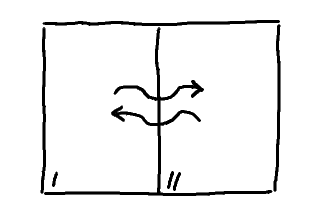
\includegraphics[width=0.4\textwidth]{osmosis}
    \caption{\textsc{The goal of osmosis is equilibrium}}
    \begin{center}I : high concentration solution\\II : low concentration solution\end{center}
  \end{figure}

  \begin{figure}[H]
    \centering
    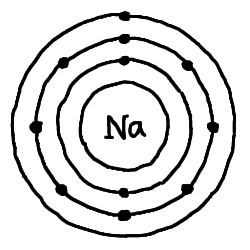
\includegraphics[width=0.25\textwidth]{rutherford}
    \caption{\textsc{Rutherford's model}}
    \begin{center}the position of electrons in layers: 2 - 8 - 18 - 32\end{center}
  \end{figure}

\end{document}
